\documentclass[a4paper]{article}

\usepackage[utf8]{inputenc}
\usepackage[T1]{fontenc}
\usepackage{textcomp}
\usepackage[english]{babel}
\usepackage{amsmath, amssymb}


%figure support
\usepackage{import}
\usepackage{xifthen}
\pdfminorversion=7
\usepackage{pdfpages}
\usepackage{transparent}
\newcommand{\incfig}[1]{%
	\def\svgwidth{\columnwidth}
	\import{./figures/}{#1.pdf_tex}
}
\graphicspath{ {./figures/} }
\pdfsuppresswarningpagegroup=1

\begin{document}
	\title{CEN4088.01 Lab 10 Due xx/xx/19}
	\author{Brandon Thompson 5517}
	\maketitle

	\begin{figure}[ht!]
		\centering
		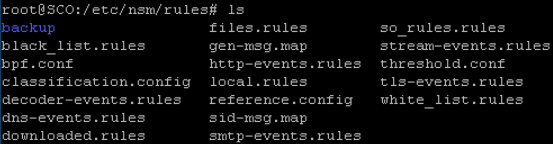
\includegraphics[width=0.8\textwidth]{1_1_15}
		\caption{Contents of \verb+/etc/nsm/rules/+ folder.}
		\label{fig:1_1_15}
	\end{figure}

	\begin{figure}[ht!]
		\centering
		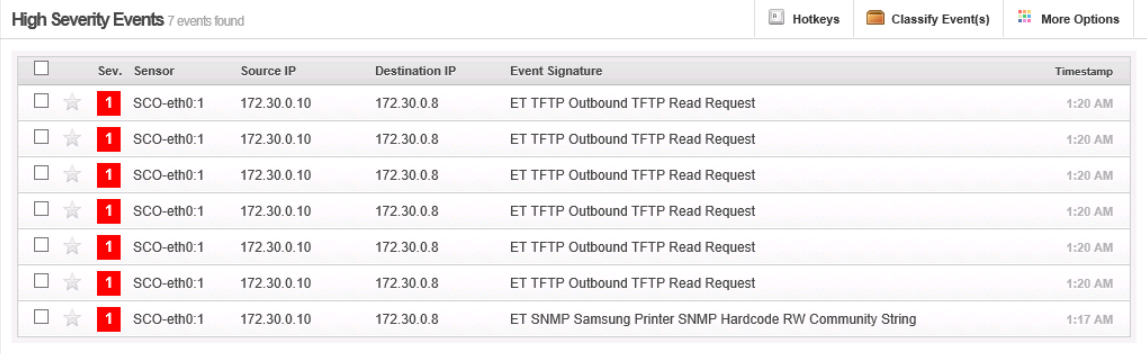
\includegraphics[width=0.8\textwidth]{1_3_3}
		\caption{Snorby list of high security vulnerabilities.}
		\label{fig:1_3_3}
	\end{figure}

	\begin{figure}[ht!]
		\centering
		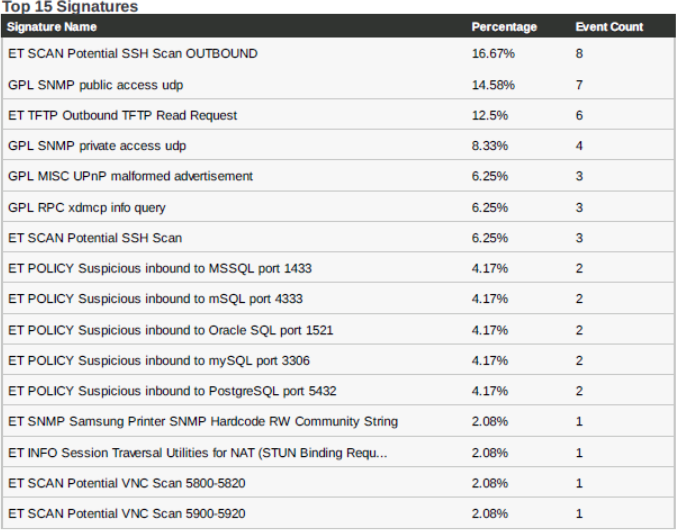
\includegraphics[width=0.8\textwidth]{1_3_13}
		\caption{Snorby top 15 signatures.}
		\label{fig:1_3_13}
	\end{figure}

	\begin{figure}[ht!]
		\centering
		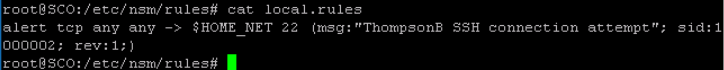
\includegraphics[width=0.8\textwidth]{2_1_18}
		\caption{Contents of \verb+/etc/nsm/rules/local.rules+ file.}
		\label{fig:2_1_18}
	\end{figure}
	
	\begin{figure}[ht!]
		\centering
		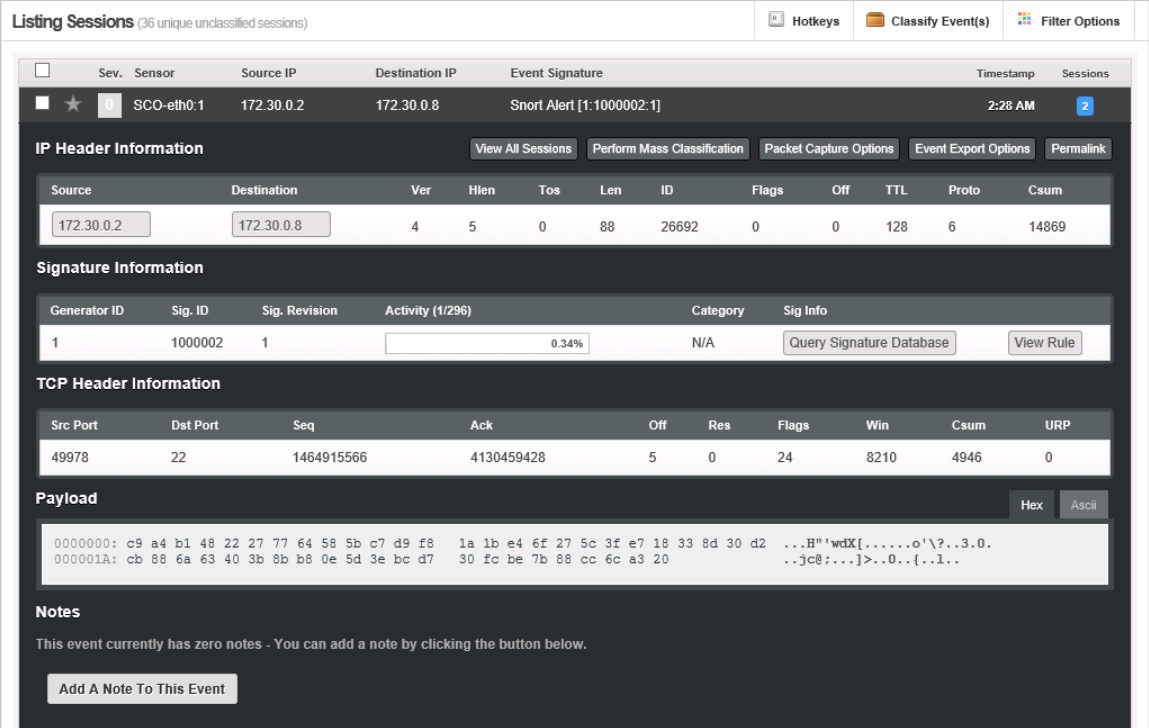
\includegraphics[width=0.8\textwidth]{2_1_26}
		\caption{Information for custom Snort alert.}
		\label{fig:2_1_26}
	\end{figure}

	\begin{figure}[ht!]
		\centering
		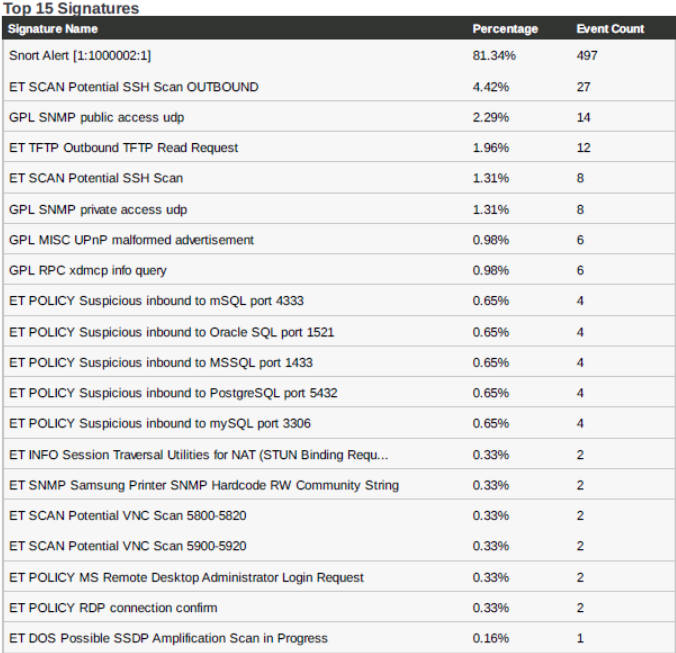
\includegraphics[width=0.8\textwidth]{2_3_7}
		\caption{Snorby top 15 signatures.}
		\label{fig:2_3_7}
	\end{figure}
	
	\begin{itemize}
		\item OS-Windows Microsoft Windows UPnP malformed advertisement: Buffer overflow in Universal
			Plug and Play (UPnP) on Windows 98,98SE, ME, and XP allows remote attackers to
			execute arbitrary code via a notify directive with a long location URL.
		\item GPL SNMP public access udp: Snort saw an SNMP packet which was accessing the "public" 
			SNMP community.
		\item ET POLICY Suspicious inbound to PostgreSQL port 5432: Snort detected suspicious activity
			associated with PostgreSQL port 5432.
	\end{itemize}
\end{document}
